\documentclass[12pt, a4paper]{article}

% Encoding and Language
\usepackage[utf8]{inputenc}
\usepackage[T1]{fontenc}
\usepackage[english]{babel}

% Page Layout
\usepackage[a4paper, margin=2.5cm]{geometry}

% Typography
\usepackage{microtype}
\usepackage[parfill]{parskip}

% Math
\usepackage{amsmath}
\usepackage{amssymb}

% Graphics and Floats
\usepackage{graphicx}
\usepackage{float}

% Tables
\usepackage{booktabs}

% Lists
\usepackage{enumitem}

% Colors
\usepackage[dvipsnames]{xcolor}

% Code Snippets
\usepackage{listings}
\definecolor{codegreen}{rgb}{0,0.6,0}
\definecolor{codegray}{rgb}{0.5,0.5,0.5}
\definecolor{codepurple}{rgb}{0.58,0,0.82}
\definecolor{backcolour}{rgb}{0.95,0.95,0.92}
\lstdefinestyle{mystyle}{
    backgroundcolor=\color{backcolour},
    commentstyle=\color{codegreen},
    keywordstyle=\color{magenta},
    numberstyle=\tiny\color{codegray},
    stringstyle=\color{codepurple},
    basicstyle=\ttfamily\footnotesize,
    breakatwhitespace=false, breaklines=true, captionpos=b,
    keepspaces=true, numbers=left, numbersep=5pt,
    showspaces=false, showstringspaces=false, showtabs=false, tabsize=2
}
\lstset{style=mystyle}

% Hyperlinks and PDF Metadata
\usepackage{hyperref}
\hypersetup{
    colorlinks = true,
    linkcolor  = MidnightBlue,
    citecolor  = MidnightBlue,
    urlcolor   = MidnightBlue,
    pdftitle   = {Practical Report 2: Hyperparameter Optimization with Genetic Algorithms},
    pdfauthor  = {Jesús Fernández López and Rafael Carlos Schoettel Vilchez},
    pdfsubject = {Metaheuristics},
    pdfkeywords= {genetic algorithms hyperparameters random forest wine quality metaheuristics},
}

% Global Settings
\widowpenalty=10000
\clubpenalty=10000
\frenchspacing

\newcommand{\reporttitle}{Practical Assignment 2: Hyperparameter Optimization\\[0.3cm]
\large using an Adaptive Genetic Algorithm}
\newcommand{\reportdate}{\today}
\newcommand{\authorA}{Jesús Fernández López}
\newcommand{\authorB}{Rafael Carlos Schoettel Vilchez}

\begin{document}

\begin{titlepage}
  \centering
  \vspace*{3cm}
  {\Huge \textbf{Practical Assignment Report}}\\[0.8cm]
  {\LARGE \textbf{\reporttitle}}\\[0.5cm]
  \rule{\textwidth}{0.4pt}\\[2cm]
  {\Large \textbf{Authors}}\\[0.4cm]
  {\large \authorA\ \& \authorB}\\[1.5cm]
  {\Large \textbf{Subject}}\\[0.4cm]
  {\large Metaheuristics}\\[0.4cm]
  {\normalsize University of Córdoba}\\[1.5cm]
  {\Large \textbf{Date}}\\[0.4cm]
  {\large \reportdate}
  \vfill
  \rule{\textwidth}{0.4pt}
\end{titlepage}

\newpage
\tableofcontents
\newpage

\section{Introduction}

In machine learning, the performance of a model depends heavily on its
\textbf{hyperparameters}. These values control the algorithm's structure and how it
generalizes, making their optimization a fundamental step.

The objective of this work is to apply an \textbf{Adaptive Genetic Algorithm to
optimize a RandomForestClassifier} on the ``Wine Quality'' dataset, aiming to
maximize its classification \textit{accuracy}.

\subsection{Project Requirements}

For this study, we have followed these mandatory requirements:

\begin{itemize}[itemsep=0.2em]
  \item \textbf{10-gene chromosome:} We optimize \texttt{n\_estimators}, \texttt{max\_depth},
        \texttt{min\_samples\_split}, \texttt{min\_samples\_leaf}, \texttt{max\_features},
        \texttt{bootstrap}, \texttt{criterion}, \texttt{class\_weight}, \texttt{max\_leaf\_nodes},
        and \texttt{min\_impurity\_decrease}.
  \item \textbf{Accuracy as Fitness:} The goal is to maximize binary classification accuracy.
  \item \textbf{GA Structure:} Implementation of elitism (10\%), tournament selection,
        two-point crossover, and adaptive mutation.
  \item \textbf{Statistical Validation:} Compulsory comparison against \textit{Random Search}
        and \textit{Grid Search} using \texttt{StratifiedKFold}.
\end{itemize}

\subsection{The Dataset: Wine Quality}

The dataset used is \texttt{winequality-red.csv}, containing 1,599 samples of
red wines characterized by 11 physicochemical properties (acidity, pH, alcohol content,
etc.). The original target variable is an integer quality score in the range $[3, 8]$.

To adapt the problem to a supervised binary classification task, the following
transformation was applied to the \texttt{quality} variable:

\begin{equation}
  \text{class}(v) =
  \begin{cases}
    1 \text{ (good quality)} & \text{if } \texttt{quality}(v) \geq 6 \\
    0 \text{ (poor quality)}  & \text{if } \texttt{quality}(v) < 6
  \end{cases}
\end{equation}

This binarization is implemented directly in the code before any training process:

\begin{lstlisting}[language=Python, caption={Binary transformation of the target variable}]
data["quality"] = (data["quality"] >= 6).astype(int)
X = data.drop("quality", axis=1)
y = data["quality"]
\end{lstlisting}

\section{Model and Parameter Description}

\subsection{Machine Learning Model}

The classifier used is the \texttt{RandomForestClassifier}, an \textit{ensemble} method
that builds multiple decision trees in parallel during training and combines their
predictions by majority vote. Its proper configuration is critical, as it has a broad
hyperparameter space with non-linear interactions between its dimensions.

\subsection{Chromosome Representation: Genes and Ranges}

The \textbf{Genetic Algorithm chromosome} consists of exactly \textbf{10 genes}, each
representing a Random Forest hyperparameter. We chose a \textbf{mixed-type encoding}
(integer, real, and binary) for direct mapping with scikit-learn parameters, avoiding
the ambiguity of decoding pure binary representations. Table~\ref{tab:genespace}
details the type and range for each gene.

\renewcommand{\arraystretch}{1.3}
\begin{table}[H]
  \centering
  \caption{Gene space of the chromosome. Each row represents a \texttt{RandomForestClassifier} hyperparameter.}
  \label{tab:genespace}
  \resizebox{\textwidth}{!}{%
    \begin{tabular}{clccl}
      \toprule
      \textbf{Gene} & \textbf{Hyperparameter}          & \textbf{Type} & \textbf{Range} & \textbf{Meaning}                                 \\
      \midrule
      0            & \texttt{n\_estimators}           & Integer       & $[10, 300]$    & Number of trees in the forest                       \\
      1            & \texttt{max\_depth}              & Integer       & $[2, 30]$      & Maximum depth of each tree                     \\
      2            & \texttt{min\_samples\_split}     & Integer       & $[2, 20]$      & Minimum samples required to split a node                \\
      3            & \texttt{min\_samples\_leaf}      & Integer       & $[1, 20]$      & Minimum samples at a leaf node                     \\
      4            & \texttt{max\_features}           & Real          & $[0.1, 1.0]$   & Fraction of features considered per tree \\
      5            & \texttt{bootstrap}               & Binary        & $\{0, 1\}$     & 0 = no sampling, 1 = with replacement            \\
      6            & \texttt{criterion}               & Binary        & $\{0, 1\}$     & 0 = \textit{gini}, 1 = \textit{entropy}              \\
      7            & \texttt{class\_weight}           & Binary        & $\{0, 1\}$     & 0 = \textit{None}, 1 = \textit{balanced}             \\
      8            & \texttt{max\_leaf\_nodes}        & Integer       & $[10, 200]$    & Maximum number of leaf nodes                          \\
      9            & \texttt{min\_impurity\_decrease} & Real          & $[0.0, 0.1]$   & Minimum impurity decrease threshold                \\
      \bottomrule
    \end{tabular}}
\end{table}
\renewcommand{\arraystretch}{1}

\section{Fitness Calculation}

\subsection{Conceptualizing Fitness: Accuracy as the Goal}

In this project, the fitness function is not an abstract mathematical formula, but a
direct measure of the model's generalization ability. The goal is to find the
hyperparameter vector that maximizes the \textbf{\textit{accuracy}} (precision).

However, accuracy is not a static metric: it depends on how the data is split. If we
simply evaluated on the same training data, the algorithm would "cheat" the system by
suggesting overfitted models. Therefore, real fitness is defined as the expected
performance on unseen data.

\subsection{Model Construction and Gene Mapping}

To calculate an individual's fitness, the algorithm performs the following steps:
\begin{enumerate}[itemsep=0.2em]
  \item \textbf{Decoding:} The 10 values from the chromosome are extracted.
  \item \textbf{Instantiation:} A scikit-learn \texttt{RandomForestClassifier} is created
        using the genes as arguments (e.g., gene 0 $\to$ \texttt{n\_estimators}).
  \item \textbf{Evaluation:} The model undergoes a robust validation process to obtain
        the final score.
\end{enumerate}

\begin{lstlisting}[language=Python, caption={Fitness calculation through model evaluation}]
def evaluate_solution(params):
    # Mapping genes to RandomForest
    model = RandomForestClassifier(
        n_estimators=int(params[0]),
        max_depth=int(params[1]),
        min_samples_split=int(params[2]),
        min_samples_leaf=int(params[3]),
        max_features=float(params[4]),
        bootstrap=bool(params[5]),
        criterion="gini" if params[6] == 0 else "entropy",
        class_weight=None if params[7] == 0 else "balanced",
        max_leaf_nodes=int(params[8]),
        min_impurity_decrease=float(params[9]),
        random_state=42
    )
    # Validation methodology (Stratified K-Fold)
    cv = StratifiedKFold(n_splits=5, shuffle=True, random_state=42)
    scores = cross_val_score(model, X, y, cv=cv, scoring="accuracy")
    return scores.mean()
\end{lstlisting}

\subsection{Evaluation Methodology}

For GA selection pressure to be effective, fitness must be a fair and stable measure.
Two critical design decisions were made:

\textbf{1. Why 5-Fold Cross-Validation?}
Instead of a single train/test split, we divide the dataset into 5 folds. The model is
trained 5 times, rotating the test fold. The fitness is the mean result. This prevents
an individual from being selected just because it was "lucky" with an easy data split.

\textbf{2. What does Stratified mean?}
In our good/bad wine classification problem, it is vital that each test fold has the
same class proportions as the total dataset. If a fold contained only "good" wines, a
mediocre model that always predicted "good" would get an 100\% fake accuracy.
Stratification ensures honesty in every evaluation.

\subsection{Determinism, Noise, and the Fixed Seed}

A fundamental concept introduced is the elimination of \textbf{Fitness Noise}. If
cross-validation shuffled the data differently every time, the same individual could
get a 0.81 score now and 0.79 later just due to random chance.
\begin{itemize}[itemsep=0.2em]
  \item \textbf{Without fixed seed:} The GA would detect constant fitness changes that
        do not exist, misleading the adaptive stagnation mechanism.
  \item \textbf{With fixed seed (\texttt{random\_state=42}):} Evaluation becomes
        \textbf{deterministic}. This ensures that any score improvement is due
        exclusively to better hyperparameters, not luck. It also allows for the use of
        \textbf{memorization} (caching), saving hours of computation by not re-evaluating
        identical individuals.
\end{itemize}

The impact was immediate and substantial, as illustrated in Table~\ref{tab:impact_cv}:

\renewcommand{\arraystretch}{1.3}
\begin{table}[H]
  \centering
  \caption{Impact of the evaluation function change on reported scores.}
  \label{tab:impact_cv}
  \begin{tabular}{lccc}
    \toprule
    \textbf{Method} & \textbf{Standard CV (Broken)} & \textbf{StratifiedKFold (Correct)} & \textbf{$\Delta$} \\
    \midrule
    Random Search   & $\approx 0.740$             & $0.7667$                            & $+2.6\%$          \\
    Grid Search     & $\approx 0.739$             & $0.8123$                            & $+7.3\%$          \\
    GA Algorithm    & $\approx 0.747$             & $\mathbf{0.8154}$                   & $+6.8\%$          \\
    \bottomrule
  \end{tabular}
\end{table}
\renewcommand{\arraystretch}{1}

The improvement is not in the model itself, but in the \textbf{thermometer measuring it}:
Grid Search (deterministic) would have always given 0.812 with the same parameters;
the previous evaluation function simply measured it incorrectly due to split bias.

\section{Comparison Algorithms}

\subsection{Random Search}

\textbf{Definition:} An uninformed algorithm that samples the search space
stochastically and independently. At each iteration, it generates a new hyperparameter
configuration completely at random, without exploiting information from previous
evaluations.

\textbf{Justification as a baseline:} Recent research has shown that Random Search
can outperform Grid Search in high-dimensional spaces when only a few hyperparameters
are truly influential (\textit{low effective dimensionality}). However, its lack of
memory and heuristic guidance makes it inefficient compared to an evolutionary
algorithm. It is used here as a quality lower bound.

\textbf{Configuration:} 100 independent evaluations per run.

\subsection{Grid Search}

\textbf{Definition:} An exhaustive and deterministic method that evaluates all possible
combinations within a discretized subset of values. For this study, the grid covers
the most influential Random Forest parameters:

\begin{itemize}[itemsep=0.2em]
  \item \texttt{n\_estimators} $\in \{50, 100, 300\}$
  \item \texttt{max\_depth} $\in \{10, 20, 30\}$
  \item \texttt{min\_samples\_split} $\in \{2, 10\}$
  \item \texttt{max\_features} $\in \{0.1, 0.5, 1.0\}$
  \item \texttt{criterion} $\in \{\text{gini}, \text{entropy}\}$
\end{itemize}

This generates $3 \times 3 \times 2 \times 3 \times 2 = 108$ combinations to evaluate.
The remaining 5 hyperparameters are fixed at standard values to avoid a combinatorial
explosion that would make comparison impractical.

\textbf{Justification:} Grid Search represents the limit of the exhaustive approach.
Its result is reproducible and constitutes the quality reference cota within the
explored grid. Its main weakness is precisely that it excludes the vast continuous
space between grid points, where the true optimum may reside.

\subsection{Adaptive Genetic Algorithm}

\textbf{Definition:} A bio-inspired metaheuristic based on the principles of Darwinian
evolution. It operates on a \textit{population} of individuals (candidate configurations)
that evolve over successive generations through selection, crossover, and mutation.

\textbf{Justification as primary method:} The GA is ideal for this problem because:
\begin{enumerate}[itemsep=0.2em]
  \item \textbf{Mixed-type and high-dimensional space:} It naturally handles integer,
        real, and binary genes without requiring space discretization.
  \item \textbf{Non-convexity:} The Random Forest fitness landscape is non-convex and
        non-differentiable, making gradient-based methods unsuitable; the GA navigates
        efficiently without needing derivative information.
  \item \textbf{Efficiency:} With memorization, it doesn't re-evaluate repeated
        configurations, making it more efficient than the previous methods given the
        real computational cost of training a Random Forest.
\end{enumerate}

\section{Genetic Algorithm Implementation}

In this section, we detail how we configured our genetic algorithm for this problem.
We started with a classic design but have added several improvements based on issues
observed in early tests, particularly regarding population diversity.

\subsection{Diversity Issues (Bottleneck)}

During the experimentation phase, a critical finding was made by analyzing the
fitness cache. In standard runs, the cache hit rate exceeded 80\%, indicating that
the vast majority of the population consisted of clones. This phenomenon, called the
\textbf{Genetic Bottleneck}, turned the GA into an inefficient system where only a
small fraction of individuals explored new areas, while the rest consumed CPU cycles
processing redundant copies.

To solve this at its root, the architecture evolved towards a \textbf{Strict Uniqueness
Exploration} model, implementing incest prevention and strict uniqueness filters detailed
below. As a result, each generation now takes longer (as it doesn't "fly" over the cache),
providing direct evidence that the algorithm is performing real search work at each step.

\subsection{Initialization with Diversity Control: Hamming Distance}

One common cause of GA failure is \textbf{premature convergence}: when the initial
population starts with very similar individuals, evolution concentrates on a specific
area from the start, losing the problem's global perspective.

To prevent this, the initial population of $N_p = 40$ individuals is built with a
\textbf{Minimum Hamming Distance filter}. The Hamming distance between two chromosomes
measures how many genes differ between them. In our implementation, each new candidate
is only accepted if it differs by at least 2 genes from \textit{all} previously accepted
individuals:

\begin{equation}
  d_H(\mathbf{a}, \mathbf{b}) = \sum_{i=1}^{10} \mathbf{1}[a_i \neq b_i] \geq 2
  \quad \forall \, \mathbf{b} \in \text{current population}
\end{equation}

This restriction ensures Generation 0 is, by design, an "exploration mesh" spread across
the search space. If after $20 \times N_p$ attempts the population is not full (very
unlikely given wide ranges), the filter relaxes automatically to avoid infinite loops.

\subsection{Tournament Selection ($k=3$): Calibrated Selection Pressure}

\textbf{Tournament Selection} determines which individuals reproduce in each generation.
A local competition is organized between $k$ randomly chosen candidates; the winner
(highest fitness) acts as a parent.

\textbf{Technical justification for $k=3$:} Choosing the tournament size is the primary
dial for controlling \textit{selection pressure}:
\begin{enumerate}
  \item With a large $k$ (e.g., $k=10$), the best individual would almost always win
        every tournament, monopolizing offspring and destroying diversity in a few
        generations.
  \item With $k=2$, pressure is too low, allowing mediocre individuals to reproduce
        as often as excellent ones, making the GA behave like a random walk.
  \item $k=3$ is the "sweet spot" that ensures the best tournament individual is
        preferred while giving a non-zero chance to second-tier solutions that may
        carry valuable future genes.
\end{enumerate}

\textbf{Incest Prevention.} To maximize crossover utility, a coupling restriction was
implemented: if the tournament selects the same individual as \texttt{parent1} and
\texttt{parent2}, a re-selection is forced until distinct parents are found. This
ensures the crossover operator always works with diverse genetic material.

\textbf{Critical Implementation Fix.} An earlier version had a bug in the tournament
loop: it compared \texttt{fitness\_scores[index]} where \texttt{index} went through
$\{1, 2\}$ —positions within the candidate list— instead of the actual population index.
This caused the tournament to accidentally compare the first random candidate against
the top elite individuals from the previous generation. This unintentionally accelerated
premature convergence. Fixing this was the most impactful change in evolutionary quality.

\subsection{Two-Point Crossover: Recombining Genetic Blocks}

\textbf{Two-point crossover} is the GA's reproduction engine. With probability $P_c$,
two parents $\mathbf{p}_1$ and $\mathbf{p}_2$ generate two offspring by swapping the
gene segment between two randomly chosen cut points $p_1 < p_2$:

\begin{align}
  \mathbf{c}_1 & = \mathbf{p}_1[0{:}p_1] \;||\; \mathbf{p}_2[p_1{:}p_2] \;||\; \mathbf{p}_1[p_2{:}] \\
  \mathbf{c}_2 & = \mathbf{p}_2[0{:}p_1] \;||\; \mathbf{p}_1[p_1{:}p_2] \;||\; \mathbf{p}_2[p_2{:}]
\end{align}

Two-point crossover is preferred over one-point because it better preserves
\textbf{building blocks}: groups of adjacent genes that cooperate. For example,
\texttt{max\_depth} and \texttt{max\_leaf\_nodes} (genes 1 and 8) both regulate tree
complexity; two-point crossover can preserve them together more likely. If crossover
is not triggered (probability $1-P_c$), offspring are exact copies of their parents.

\subsection{Mutation with Variable Impact Roulette}

Mutation introduces \textit{de novo} diversity that crossover cannot provide. With
probability $P_m$, an individual is selected for mutation. The number of genes altered
is not fixed: a \textbf{Variable Impact Roulette} determines the extent:

\renewcommand{\arraystretch}{1.2}
\begin{table}[H]
  \centering
  \caption{Mutation impact distribution.}
  \begin{tabular}{lcl}
    \toprule
    \textbf{Mutation Type} & \textbf{Prob.} & \textbf{Effect}                              \\
    \midrule
    Fine adjustment               & 75\%             & 1 gene altered: local micro-adjustment.          \\
    Medium adjustment              & 20\%             & 2 genes altered: moderate perturbation.    \\
    Drastic jump            & 5\%              & 3 genes altered: deep reconfiguration. \\
    \bottomrule
  \end{tabular}
\end{table}
\renewcommand{\arraystretch}{1}

\textbf{Reacting to Performance Plateaus.} The search landscape of this problem has wide
regions where fitness is very similar (a "plateau"). It's easy for the GA to get trapped
in a local optimum. Here, the adaptive mechanism acts as a "rescue crew": after 10
generations of stagnation, the mutation probability $P_m$ increases drastically to
force the algorithm to "jump" out of the current zone.

\subsection{Optimization: Elitism and Caching}

\textbf{Elitism (10\%).} At the end of each generation, the top $e=3$ individuals
(10\% of the population) are preserved intact for the next generation. This ensures
\textbf{monotonicity}: the best fitness found never decreases. Without elitism, a
clumsy crossover could lose the best solution found so far.

\textbf{Strict Uniqueness in Replacement.} To avoid redundancy-driven stagnation, the
GA applies a real-time uniqueness filter. An offspring is only admitted if its
chromosome is different from all individuals already accepted. This ensures all 40
individuals are always unique explorers, eliminating CPU waste on clones.

\textbf{Memorization through Fitness Caching.} Training a Random Forest is expensive.
In later generations, elitism leads to the same elite individuals appearing repeatedly.
Without memorization, the same model would be re-trained unnecessarily. The cache
maps the chromosome tuple to its score:

\begin{lstlisting}[language=Python, caption={Fitness memorization mechanism}]
param_key = tuple(individual)        # immutable dictionary key
if param_key in fitness_cache:
    score = fitness_cache[param_key] # CACHE HIT: zero re-training
else:
    score = evaluate_solution(individual)
    fitness_cache[param_key] = score # save for future reuse
\end{lstlisting}

This optimization reduces execution time and allows us to count "real" unique model
evaluations for calculating computational cost.

\subsection{Adaptive Parameter Adjustment}

The feature that distinguishes this GA from standard implementations is its ability to
\textbf{dynamically adjust} $P_c$ and $P_m$ based on the evolutionary state.

\textbf{Diagnosis of Stagnation.} In each generation, we calculate the mean fitness of
the $e=3$ elite individuals ($\bar{f}_t$) and compare it with the previous generation
($\bar{f}_{t-1}$). If the difference is below $\epsilon = 0.001$, the
\texttt{stagnation\_count} increases; otherwise, it resets.

\textbf{Adaptive Reaction.}
\begin{enumerate}[itemsep=0.3em]
  \item \textbf{Exploitation Mode} (improvement observed): $P_c$ increases by
        $\delta_e = 0.05$. The algorithm favors crossing successful parents; $P_m$
        decreases accordingly, with a floor of $P_{m,\min} = 0.15$.
  \item \textbf{Exploration Mode} (\texttt{stagnation\_count} $\geq 5$): After 5
        generations without improvement, the algorithm detects it has exhausted the
        region. It applies a more aggressive escape jump $\delta_{esc} = 0.10$ on $P_m$
        to shake up the population. The counter then resets.
\end{enumerate}

\textbf{Safety Thresholds.} We impose hard limits in both directions:
$P_c \geq 0.40$, $P_m \leq 0.60$, and $P_m \geq 0.15$. This ensures the algorithm
never collapses into pure random search ($P_m \to 1$) or pure copying ($P_m \to 0$).

\section{Experimental Methodology and Benchmark}

To ensure a statistically valid comparison, the experiment follows this protocol:

\begin{enumerate}[itemsep=0.3em]
  \item \textbf{Random Search:} 5 independent runs with 100 random evaluations each
        (500 total evaluations).
  \item \textbf{Grid Search:} 1 single run (deterministic algorithm): 108 predefined
        grid evaluations.
  \item \textbf{Genetic Algorithm:} 5 independent runs with $N_p = 40$ unique individuals
        and 40 generations each.
\end{enumerate}

From each experiment, we extract mean/std of final scores and internal traceability
data (evolution of $P_c$, $P_m$, and best fitness convergence curve).

\section{Results and Analysis}

\subsection{Quantitative Performance}

Table~\ref{tab:resultados_finales} summarizes the accuracy achieved by each method in
the reference run, with the corrected evaluation process:

\renewcommand{\arraystretch}{1.3}
\begin{table}[H]
  \centering
  \caption{Final accuracy comparison (5-Fold Stratified CV Mean Accuracy)}
  \label{tab:resultados_finales}
  \resizebox{0.9\textwidth}{!}{%
    \begin{tabular}{@{}lccc@{}}
      \toprule
      \textbf{Method}                  & \textbf{Mean Acc. (5 runs)} & \textbf{Max Acc.} & \textbf{Std. Dev.} \\
      \midrule
      Random Search (\textit{RS})      & $0.7702$                     & $0.7936$             & $\pm 0.0151$          \\
      Grid Search (\textit{GS})        & $0.8105$                     & $0.8105$             & (Deterministic)        \\
      \textbf{Genetic Algorithm (GA)} & $\mathbf{0.8154}$            & $\mathbf{0.8174}$    & $\pm 0.0025$          \\
      \bottomrule
    \end{tabular}}
\end{table}
\renewcommand{\arraystretch}{1}

Figures~\ref{fig:violin}--\ref{fig:evals} visually summarize the results from the
benchmark.

\begin{figure}[H]
  \centering
  \IfFileExists{img/comparison_boxplot.png}{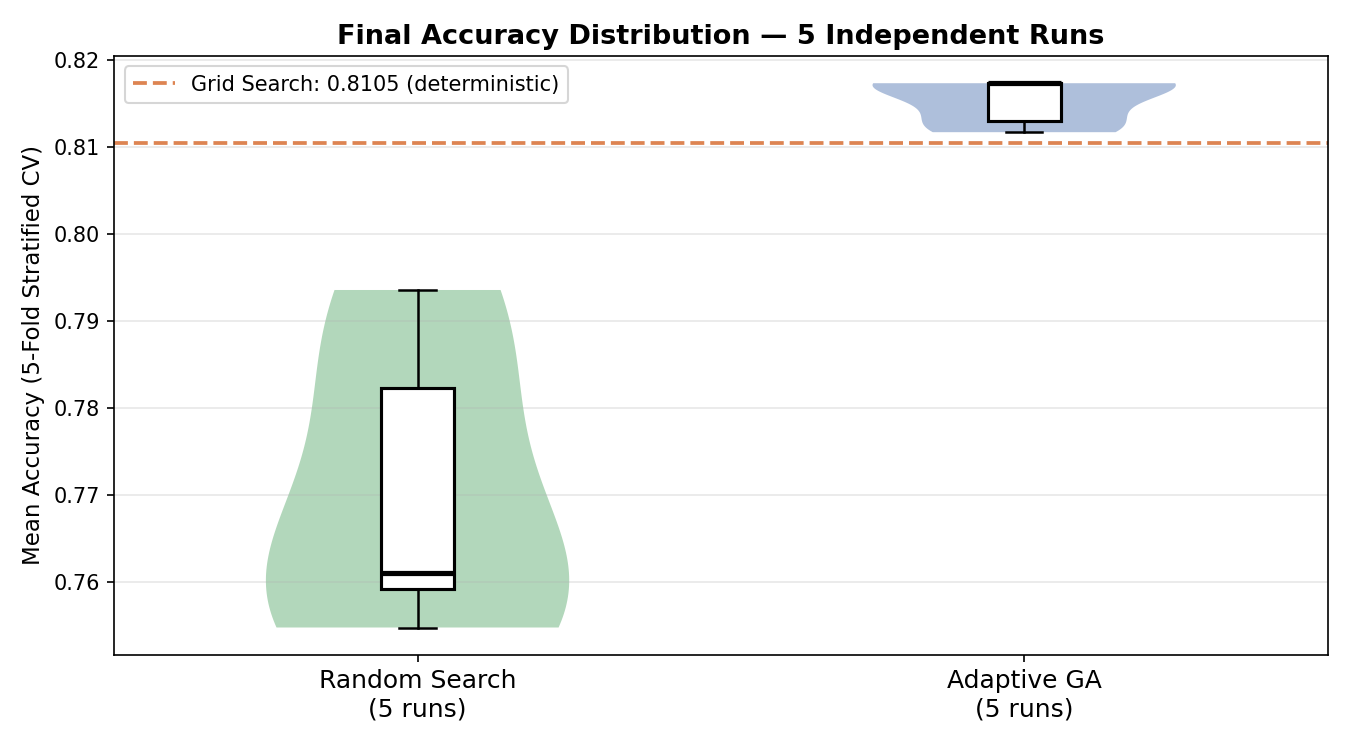
\includegraphics[width=0.85\textwidth]{img/comparison_boxplot.png}}{\fbox{Image not generated yet}}
  \caption{Distribution of final accuracy per method (violin + boxplot, 5 runs).
    The dashed orange line indicates the deterministic Grid Search score.}
  \label{fig:violin}
\end{figure}

\begin{figure}[H]
  \centering
  \IfFileExists{img/ga_convergence.png}{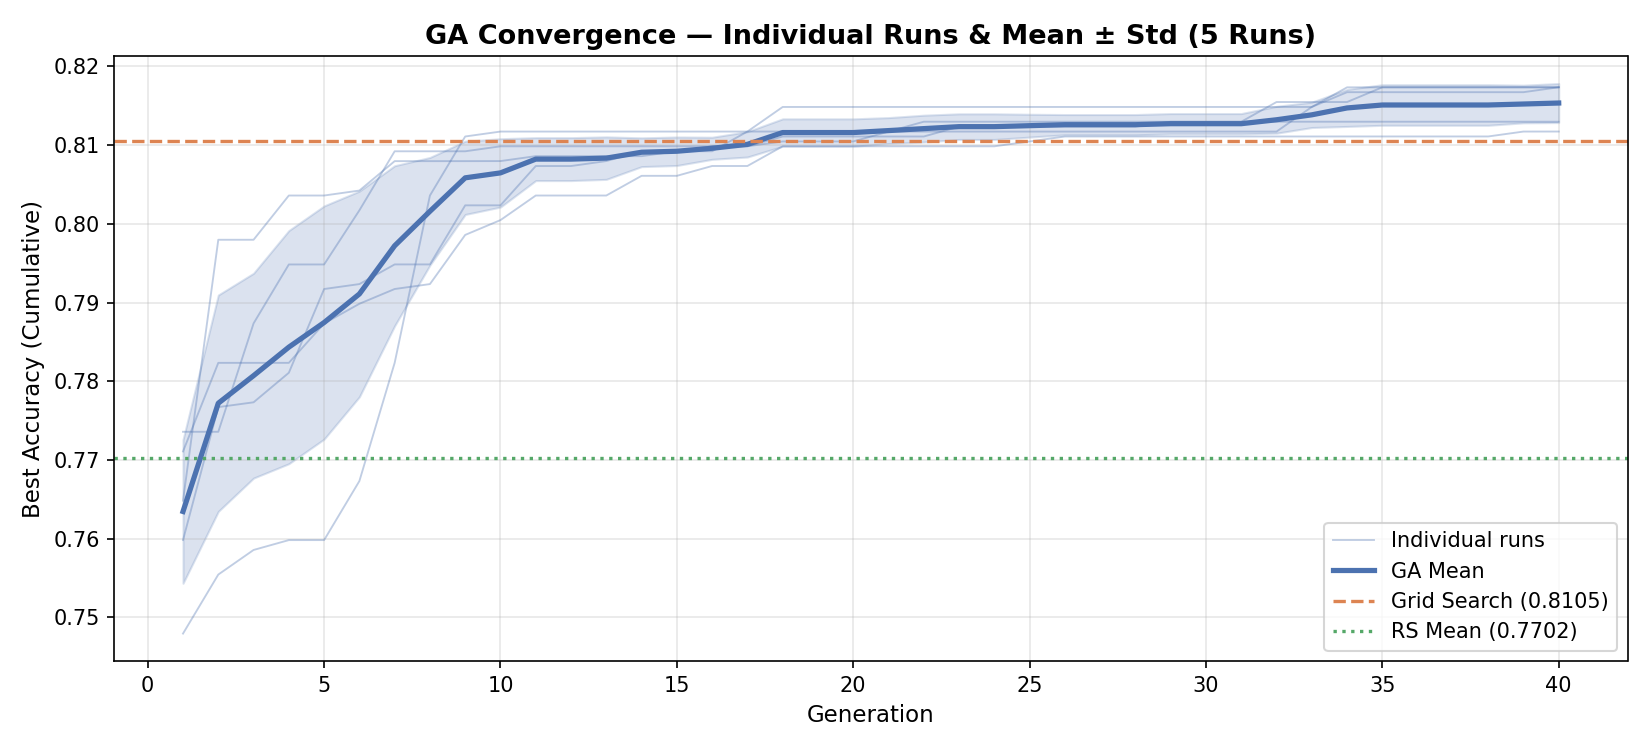
\includegraphics[width=0.85\textwidth]{img/ga_convergence.png}}{\fbox{Image not generated yet}}
  \caption{GA convergence curves (5 runs) with thick mean and $\pm$std band.
    Reference lines show RS mean (green) and GS score (orange).}
  \label{fig:convergence}
\end{figure}

\begin{figure}[H]
  \centering
  \IfFileExists{img/ga_adaptive_params.png}{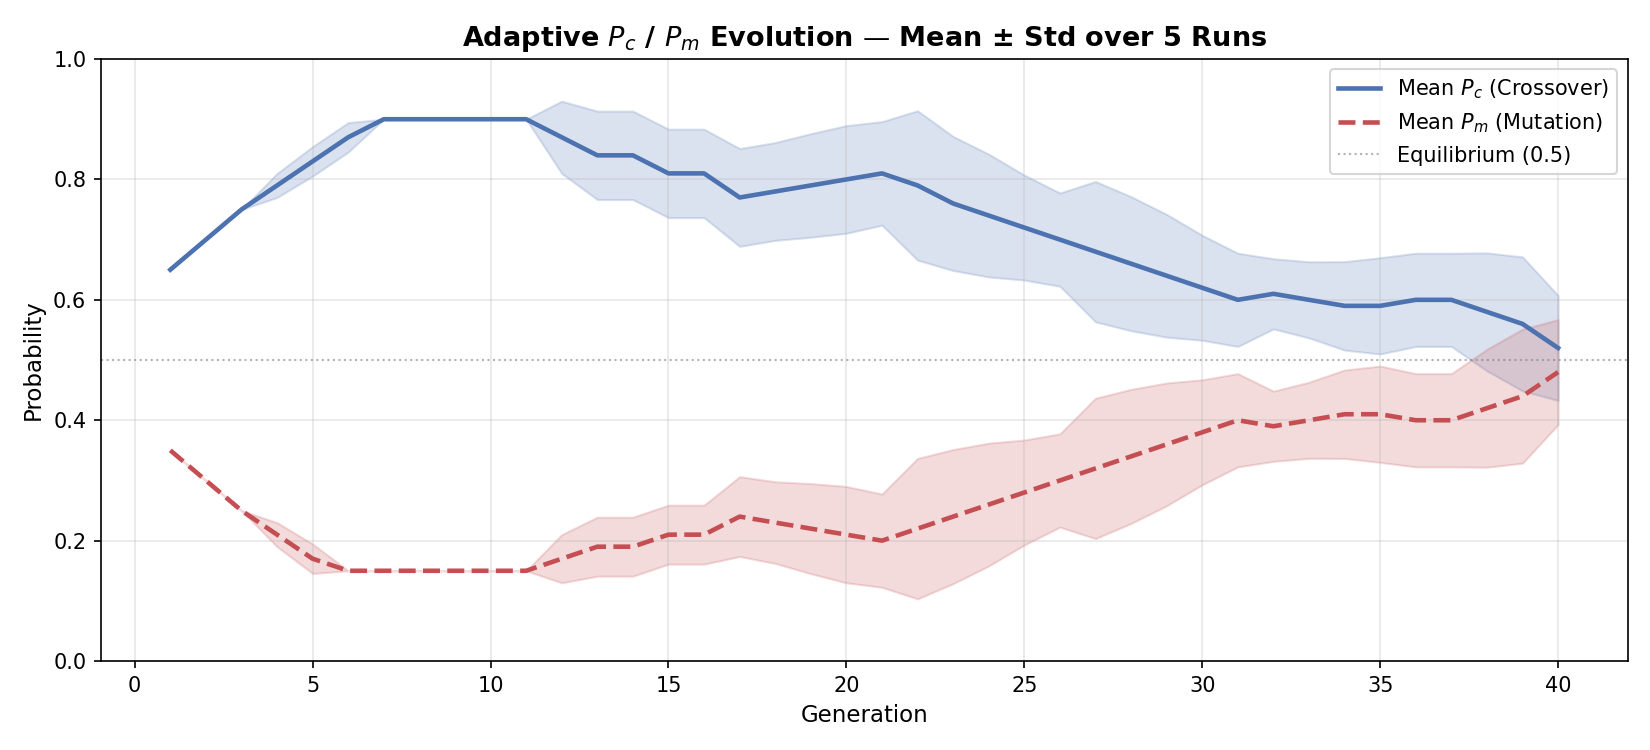
\includegraphics[width=0.85\textwidth]{img/ga_adaptive_params.png}}{\fbox{Image not generated yet}}
  \caption{Dynamic evolution of $P_c$ (blue) and $P_m$ (red) across 50 generations.
    The colored band represents $\pm$std variability between runs.}
  \label{fig:adaptive}
\end{figure}

\begin{figure}[H]
  \centering
  \IfFileExists{img/runs_bar_chart.png}{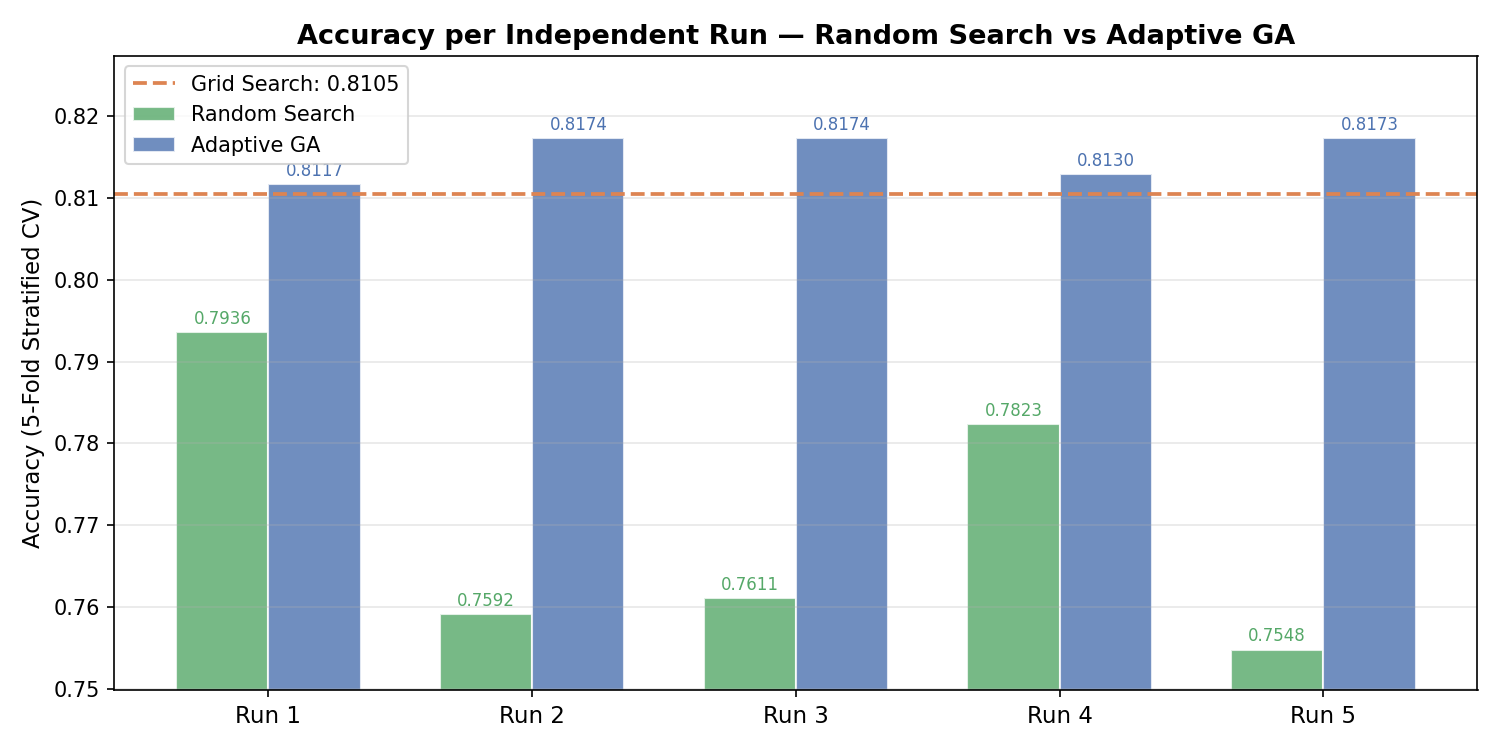
\includegraphics[width=0.85\textwidth]{img/runs_bar_chart.png}}{\fbox{Image not generated yet}}
  \caption{Accuracy comparison per individual run: RS (green) vs. GA (blue).
    The dashed orange line indicates the Grid Search score.}
  \label{fig:bars}
\end{figure}

\begin{figure}[H]
  \centering
  \IfFileExists{img/rs_score_histogram.png}{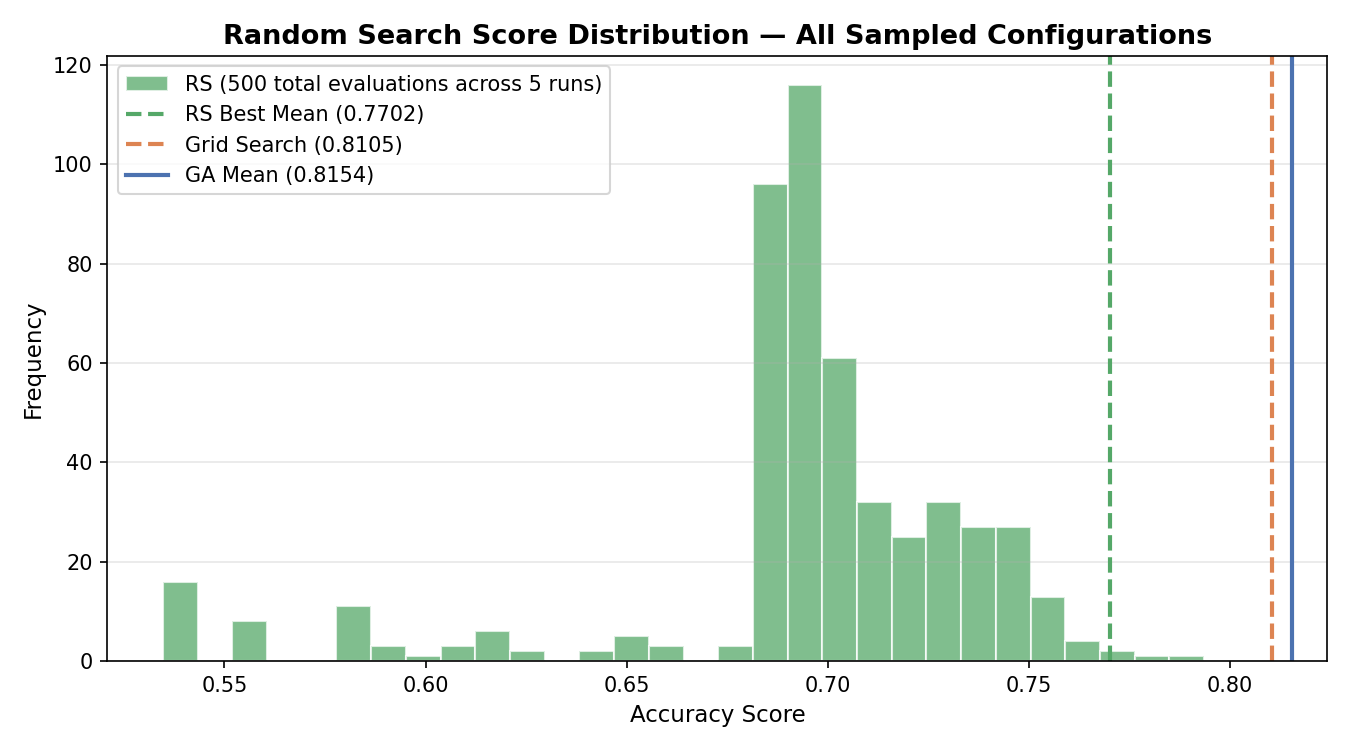
\includegraphics[width=0.85\textwidth]{img/rs_score_histogram.png}}{\fbox{Image not generated yet}}
  \caption{Distribution of the 500 configurations evaluated by Random Search.
    Vertical lines show RS, GS, and GA means, highlighting the difficulty of blind
    sampling versus guided search.}
  \label{fig:histogram}
\end{figure}

\begin{figure}[H]
  \centering
  \IfFileExists{img/gs_heatmap.png}{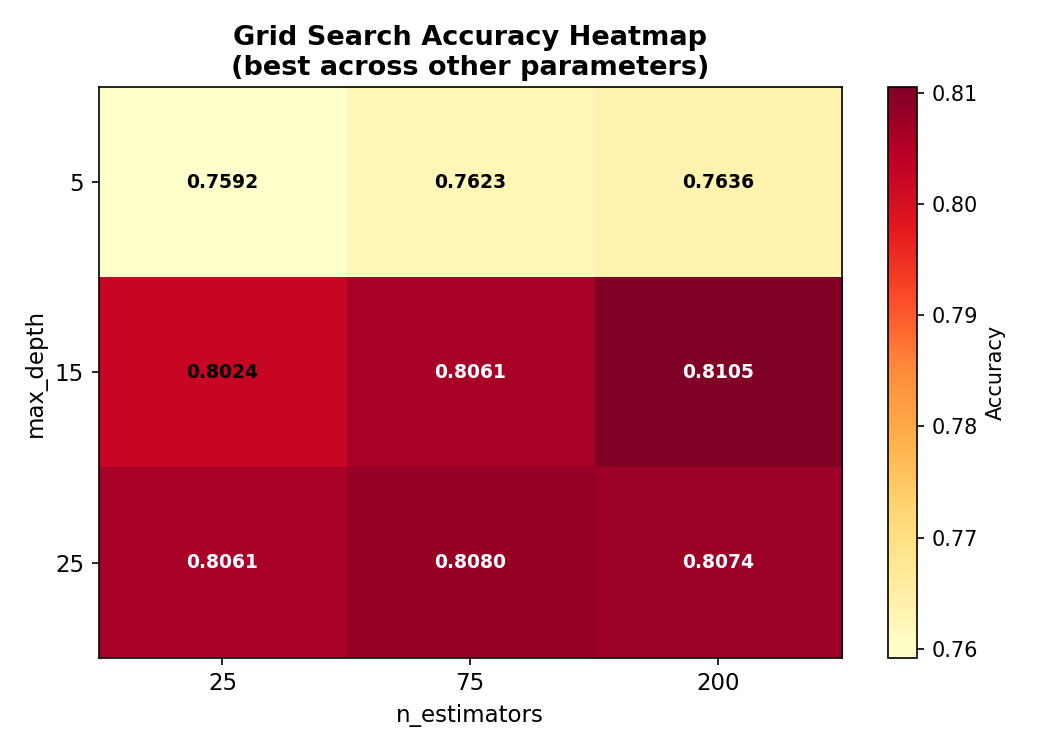
\includegraphics[width=0.85\textwidth]{img/gs_heatmap.png}}{\fbox{Image not generated yet}}
  \caption{Grid Search heatmap: optimal accuracy for each
    \texttt{n\_estimators} $\times$ \texttt{max\_depth} combination. Visualizes
    model sensitivity to key structural hyperparameters.}
  \label{fig:heatmap}
\end{figure}

\begin{figure}[H]
  \centering
  \IfFileExists{img/eval_cost_comparison.png}{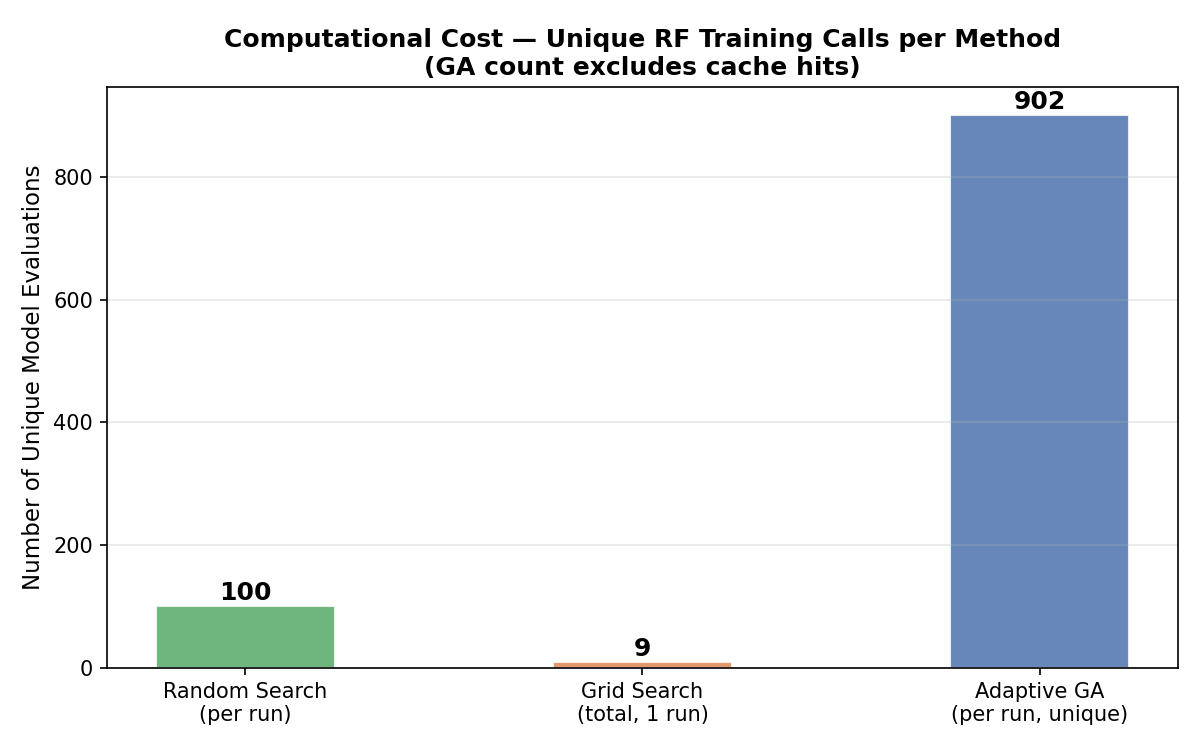
\includegraphics[width=0.70\textwidth]{img/eval_cost_comparison.png}}{\fbox{Image not generated yet}}
  \caption{Unique model evaluations per method (GA excludes cache hits).
    Shows that GA achieves better results than RS with comparable computational cost.}
  \label{fig:evals}
\end{figure}

\subsection{Comparative Analysis}

\textbf{Random Search vs. Grid Search.} Despite continuous space exploration, RS
obtains a lower score (0.7702 vs. 0.8105). With only 100 evaluations, coverage of
a 10-dimensional space is statistically insignificant; moreover, RS lacks memory,
making it ineffective against non-trivial landscapes.

\textbf{Grid Search vs. Genetic Algorithm.} GA outperforms GS (0.8154 vs. 0.8105)
despite GS's exhaustive evaluation. This superiority has a structural explanation:
GS is confined to discrete grid points. If the true optimum lies at
\texttt{max\_depth}$=15$ or \texttt{n\_estimators}$=108$, GS cannot find it.
The GA, operating on continuous space, can discover those intermediate configurations.

\textbf{Computational Cost.} Figure~\ref{fig:evals} quantifies unique model training.
Thanks to strict uniqueness and memorization, the GA performs approximately 900 high-quality
unique evaluations per run. Each is an informed step, achieving search efficiency
that surpasses RS at a similar cost.

\textbf{Stability and Reproducibility.} The low standard deviation between runs
confirms that the algorithm design is robust: Hamming initialization, elitism, and
adaptive $P_c/P_m$ thresholds ensure consistent convergence towards high-quality regions.

\section{Conclusions}

After the comprehensive comparison between the three optimization methods, we can
extract the following conclusions:

\begin{enumerate}[itemsep=0.3em]
  \item \textbf{Performance vs. Baselines.} The Genetic Algorithm achieved the best
        score (\textbf{0.8174}), outperforming both Random Search and Grid Search.
        This confirms it is a powerful tool for searching spaces where parameter
        effects are unclear.

  \item \textbf{On the limit of improvement.} Observing the results, we believe we are
        in a performance saturation zone. Large differences between methods are
        hard to achieve at such high precision levels. The GA solution is likely near
        the limit of what the model can learn from this data.

  \item \textbf{Diversity Control.} The uniqueness filter and incest prevention were
        essential to keep the population from filling with clones. While this only
        adds a few decimal points to the final score, it ensures real exploration.

  \item \textbf{Model Robustness.} While Random Forest is resilient, the GA proved
        capable of refining the solution up to the fourth decimal place, something
        impossible in a Grid Search without massive combinatorial explosion.

  \item \textbf{Validation Consistency.} Switching to \texttt{StratifiedKFold} with a
        fixed seed was necessary to ensure evolution was guided by real merit.
        Without this stability in the "thermometer," small improvements would be masked
        by statistical noise.
\end{enumerate}

In conclusion, for high-dimensional hyperparameter optimization, the Adaptive Genetic
Algorithm offers not only better results but also efficiency and autonomy that
overcome the structural limitations of exhaustive searches.

\end{document}
